\documentclass{article}

\usepackage{../preamble}
\standalonetrue

\pagestyle{fancy}
\fancyhf{}
\rhead{Section \thesection}
\lhead{PHYS 304 Lecture !!!}
\rfoot{Page \thepage}


\title{PHYS 304 Lecture 06}
\author{Ashtan Mistal}
\date{!!!}

\begin{document}

\ifstandalone
\maketitle
\fi

\graphicspath{{./Lecture06/}}


\section{Review of key points from last day}

The normalized solution of the time independent Schrodinger equation for an infinite square well potential outside of $0 < x < a$, the $\psi_n(x) - \sqrt{\frac{2}{a}} \sin \left( \frac{n \pi x}{a} \right)$ for $n = 1,2,...$ form an orthonormal and complete set of functions in the region $0 < x < a$, that are zero at the boundaries. 

\section{Recipe for solving the full Schrodinger Equation}

Solve a dynamical problem where the wavefunction is not just a stationary eigenstate. 

The following is the \textit{instruction manual} for quantum mechanics. For the rest of the course, we have to get our heads around all its implications, and learn how to actually solve for the time-independent solutions in different cases. Absolutely crucial that the $c$’s are all constant!!!

The algorithm (flowchart) for solving the full Schrodinger equation using separation of variables:


\begin{figure}[h]
    \centering
    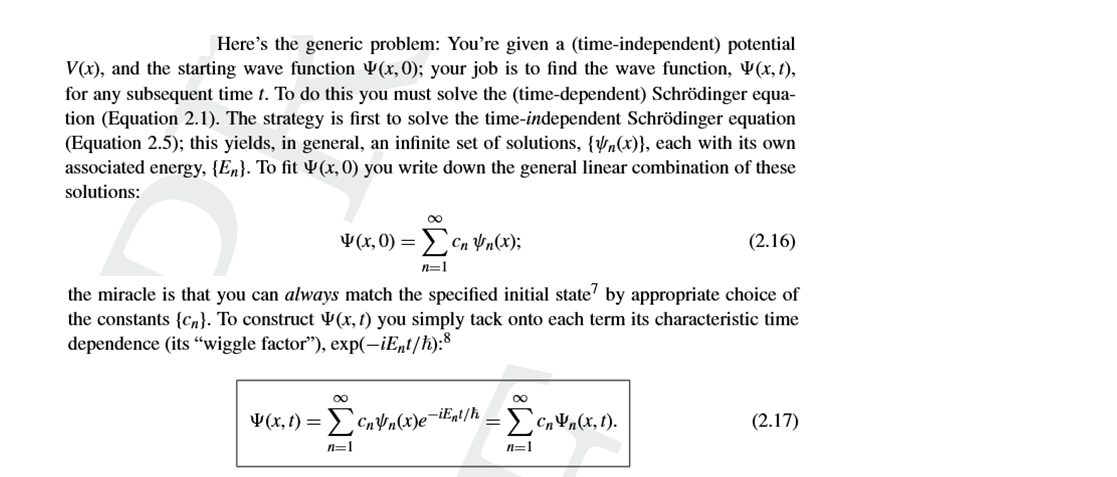
\includegraphics[width =  \textwidth]{Lecture06/1.png}
    \caption{Caption}
    \label{fig:my_label}
\end{figure}

What has gone on here?

\begin{enumerate}
    \item We assumed that there is a separable solution to the full SE
    \item Derived 2 differential equations [ordinary] that seem easier to solve than one PDE
    \item Assume that these can be solved for an intimately connected pair of spatial and temporal functions that can each be normalized for an infinite set of values of $E_n$
    \item Take it on faith from mathematicians that a general solution of the full SE can always be expanded as a linear combination of these stationary solutions, \textbf{with constant coefficients} that can be determined by knowing the spatial variation of the full wavefunction at any specific time.
\end{enumerate}

Now, let's complete the story for the infinite square well potential:

The recipe for obtaining the expansion coefficients, $c_n$, is:

$$c_n = \int_0^a \psi_n^* (x) \Psi(x,0) dx$$

Using thus with our solutions for the infinite well stationary states we then get:

$$\Psi(x,t) = \sum_{n=1}^\infty c_n \sqrt{\frac{2}{a}} \sin \left( \frac{n \pi x}{a} \right) e^{-i (n^2 \pi^2 \hbar)/(2ma^2)(t - t_0)}$$

for $t > t_0$. 

Hence, 

$$\Psi(x,t) = \sum_{n=1}^\infty \left[  \int_0^a \psi_n^* (x) \Psi(x,0) dx \right] \sqrt{\frac{2}{a}} \sin \left( \frac{n \pi x}{a} \right) e^{-i (n^2 \pi^2 \hbar)/(2ma^2)(t - t_0)}$$

for $t > t_0$. 

This equation is general, for any potential, if the range of integration goes from $-\infty$ to $\infty$. The equation for $c_n$ is equivalent to the dot product in 2D real vector space. 

\section{Dynamics of an electron in an infinite square well}

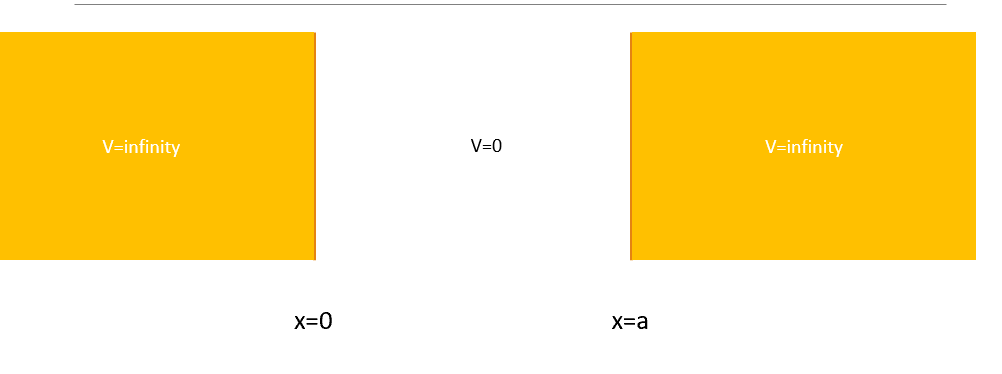
\includegraphics[width = \textwidth]{Lecture05/4.png}

Take the initial ($t_0 = 0$) wavefunction of the particle in an infinite square potential to be an equally weighted superposition of the lowest two stationary states:

$$\Psi(x,t=0) = \frac{1}{\sqrt{2}} \left( \psi_1(x) + \psi_2(x) \right)$$

Let's study the state evolution as a function of time (i.e. dynamics of an electron in this state at $t = 0$):

Explicitly, this corresponds to some initial (at $t=0$) wavefunction that just so happens to have only 2 non-zero inner product integrals with all of the  (infinite in number) bases states. 

\subsection{Activity 1}

What are the coefficients $c_1$ and $c_2$ in the general form solution?


$$\Psi(x,t) = \sum_{n=1}^\infty c_n \sqrt{\frac{2}{a}} \sin \left( \frac{n \pi x}{a} \right) e^{-i (n^2 \pi^2 \hbar)/(2ma^2)(t - t_0)}$$

\emph{See special lecture notes on Canvas: Infinite\_well\_dynamics\_2021.pdf}. 

\subsection*{Sanity Check}

Is our answer for the effective distance the particle travels from left to right reasonable?


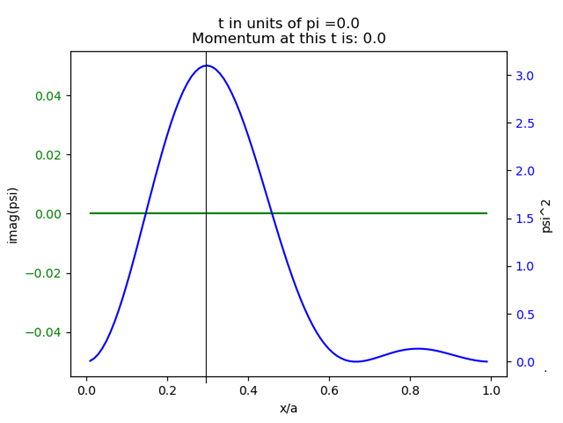
\includegraphics[width = 0.7 \textwidth]{Lecture06/2.png}




\end{document}